\subsection{Réalisation de l'analyse Entité-Relation}

\subsubsection{Entités}

Nous avons pu identifier les entités suivantes :
\begin{itemize}
  \itemperso{Utilisateur}Chaque client doit être enregistré dans la base de données et dispose des champs suivants :
  \begin{itemize}
    \subitemperso{Nom}Son nom.
    \subitemperso{Mail}Une adresse mail.
    \subitemperso{Adresse}Une adresse pour la facturation.
    \subitemperso{Mot de passe} Un mot de passe pour l'identification lors de la connexion.
  \end{itemize}
  \itemperso{Achat}Achat d'un téléphone, d'une formule ou les deux. Ils ont chacun :
  \begin{itemize}
    \subitemperso{Date} Une date d'achat
    \subitemperso{Téléphone} Le téléphone acheté
    \subitemperso{Formule} La formule achetée
    \subitemperso{Utilisateur} L'utilisateur qui a fait l'achat
  \end{itemize}
  \itemperso{Consommation} Identifie l'ensemble des consommations effectuées par un utilisateur avec un forfait sur une période donnée.
  \begin{itemize}
    \subitemperso{Date début}Date de début de la période d'enregistrement (période de 1 mois)
    \subitemperso{Consommation Données}Le montant de données consommées sur le mobile
    \subitemperso{Achat}L'achat avec lequel a été réalisé cette consommation
  \end{itemize}
  \itemperso{SMS et MMS} Les SMS et MMS envoyés ont les propriétés suivantes :
  \begin{itemize}
    \subitemperso{Date} La date et l'heure d'envoi
    \subitemperso{Volume} Le nombre de SMS/MMS correspondant au message envoyé
    \subitemperso{Destination} Le pays de destination du SMS/MMS
    \subitemperso{Consommation} La consommation à laquelle ce message est rattaché
  \end{itemize}
  \itemperso{Appel} Les appels émis ont les propriétés suivantes :
  \begin{itemize}
    \subitemperso{Date} La date et l'heure du début de l'appel
    \subitemperso{Durée} La durée de l'appel
    \subitemperso{Destination} Le pays de destination de l'appel
    \subitemperso{Consommation} La consommation à laquelle cet appel est rattaché
  \end{itemize}
  \itemperso{Facture} Les factures des clients ont les propriétés suivantes :
  \begin{itemize}
    \subitemperso{Prix} Le montant de la facture
    \subitemperso{Payé} Si le client a payé ou non cette facture
    \subitemperso{Consommation} La consommation à laquelle cette facture est rattaché
  \end{itemize}
  \itemperso{Téléphone} Tous les modèles de téléphones en vente et leurs caractéristiques :
  \begin{itemize}
    \subitemperso{Ecran}
    \subitemperso{Technologie Internet}
    \subitemperso{TV}
    \subitemperso{Appareil Photo}
    \subitemperso{RAM}
    \subitemperso{Stockage}
    \subitemperso{Carte SD}
    \subitemperso{Double SIM}
    \subitemperso{Photo}
    \subitemperso{Modele}
    \subitemperso{Marque}
    \subitemperso{Prix}
  \end{itemize}
  \itemperso{Formule} Tous les forfaits en vente disposent de :
  \begin{itemize}
    \subitemperso{Nom} Le nom du forfait
    \subitemperso{Prix} Le prix du forfait
    \subitemperso{Limite d'appel, SMS et data} Une limite pour les sms, les appels (en durée) et les données internet (en Mo).
    \subitemperso{Plage Horaire} Plage dans laquelle les communications sont gratuites
    \subitemperso{Prix hors forfait} Différent pour les appels, les SMS et les données.
    \subitemperso{Bloqué} Si le forfait est bloqué ou non
  \end{itemize}
  \itemperso{Forfait étranger} Conditions tarifaires pour la communication vers un pays ce qui comprend les même conditions qu'une formule plus :
  \begin{itemize}
    \subitemperso{Destination} La zone géographique correspondant à ce forfait étranger
  \end{itemize}
  \itemperso{Promotion} Une promotion sur une formule
  \begin{itemize}
    \subitemperso{Prix de base}
    \subitemperso{Nouveau prix}
    \subitemperso{Téléphone} Eventuellement un autre téléphone
    \subitemperso{Date de début} Début de la promotion
    \subitemperso{Durée} Durée de la promotion
  \end{itemize}
  \itemperso{Plage Horaire} Définit une période dans la semaine
  \begin{itemize}
    \subitemperso{Nom} Nom associé à la plage horaire pour plus de clarté
    \subitemperso{Heure de début}
    \subitemperso{Heure de fin}
    \subitemperso{Jour} Les jours de la semaine concernés
  \end{itemize}
  \itemperso{Zone géographique} Définit une partie du monde
  \begin{itemize}
    \subitemperso{Nom}
  \end{itemize}
  \itemperso{Pays} Les pays du monde
  \begin{itemize}
    \subitemperso{Nom}
  \end{itemize}
\end{itemize}

\begin{figure}[ht]
  \centering
    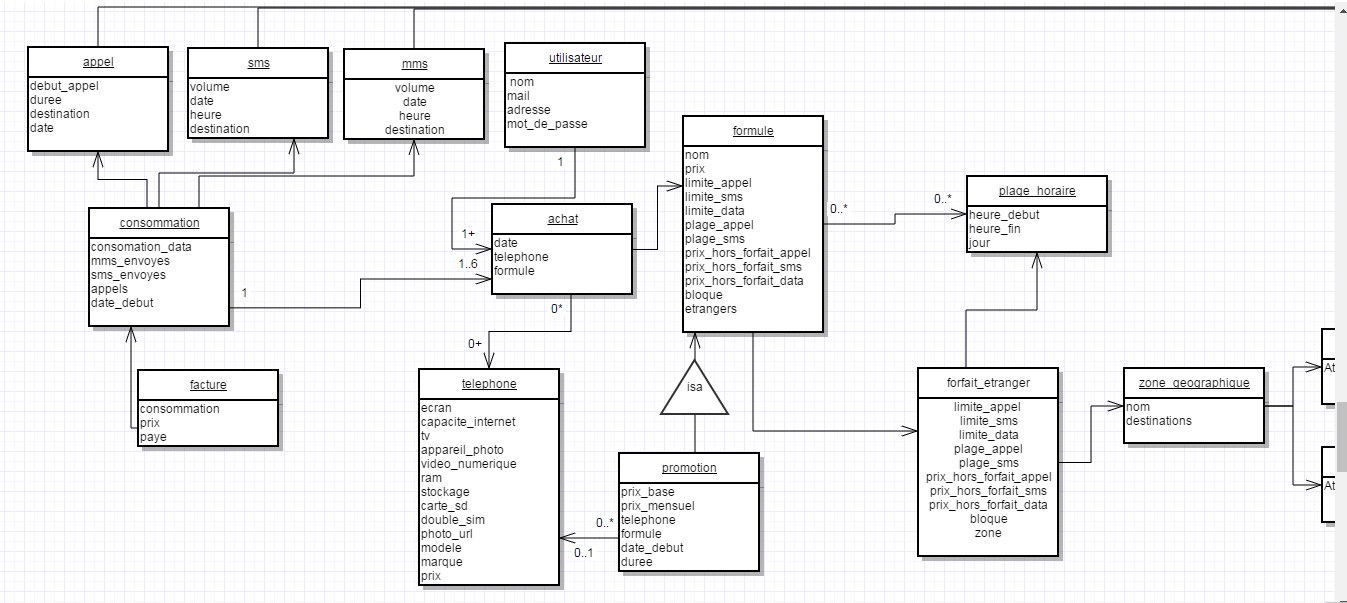
\includegraphics[width=.9\textwidth]{images/Elaboration/diagramme}
    \caption{Le diagramme Entité-Relation de notre base de données}
    \label{fig:diagrammeER}
\end{figure}


\subsubsection{Les Relations}
Certaines relations \texttt{1..N} ont déjà été mentionnées ci-dessus.
Les relations \texttt{N..N} sont les suivantes :
\begin {itemize}
  \itemperso{Formule - Plage Horaire}
  \itemperso{Forfait Etrangers - Plage Horaire}
  \itemperso{Formule - Forfait Etrangers}
  \itemperso{Formule - Téléphone}
  \itemperso{Zone Géographique - Pays}
\end {itemize}


\subsubsection{Implémentation}
Toutes les entités donneront lieu à des tables à l'exception de Promotion qui est une spécialisation de Formule. On ajoute alors les champs spécifiques à Promotion dans Formule sans toujours les utiliser.
Toutes les relations \texttt{N..N} donnent également lieu à des tables d'associations.

Cette vision est résumée par le diagramme Entité-Relations présentés en Figure~\ref{fig:diagrammeER}.


%%% Local Variables:
%%% mode: latex
%%% TeX-master: "../../Rapport_BDD"
%%% End:
